\scanpage{124}
% archive sheet number: 123
% source lines 1--18
the functor compatible with the associative unital $\unsure{\otimes|\Omega}$ that one obtains from $C$ to $\mathrm{Rep}_k(G)$, and see in particular under what conditions it is an equivalence of categories: \deleted{Then}\inserted{\handwritten{it is necessary and \unsure{p.|sufficient} that $A$ be commutative! ``Geometrically''}\handwritten{\begin{tikzpicture}[x=.4cm,y=.4cm,baseline=-.2ex]\draw (0,-.55) .. controls (-.12,.02) and (.12,.28) .. (.42,.30)--(6.8,.30) .. controls (7.04,.30) and (7.18,.36) .. (7.18,.54);\end{tikzpicture}}} When this is so,\inserted{\handwritten{\uuline{in the graded anticommutative case}}\handwritten{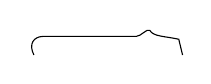
\begin{tikzpicture}[x=.4cm,y=.4cm,baseline=-.2ex]\draw (0,-.30) .. controls (-.18,.06) and (0,.28) .. (.28,.29)--(3.25,.29) .. controls (3.40,.29) and (3.58,.55) .. (3.68,.48) .. controls (3.80,.28) and (4.15,.30) .. (4.60,.20)--(4.72,-.30);\end{tikzpicture}}} \rlap{k}the situation is described entirely by the data of $G$, of the grading on \deleted{its} the forgetful functor on \deleted{$C$}\inserted{$R_k(G)$\handwritten{\begin{tikzpicture}[x=.4cm,y=.4cm,baseline=-.2ex]\draw (0,-.48) .. controls (-.12,.0) and (.15,.12) .. (.42,.14)--(1.38,.14) .. controls (1.56,.16) and (1.64,.24) .. (1.65,.43);\end{tikzpicture}}}, described by a homomorphism of monoids $\underline{G}_m\handwritten{\to}G$, and finally the condition that for two representations $M,N$ of $G$, the Koszul isomorphism $M\otimes N\handwritten{\xrightarrow{\sim}}N\otimes M$ on the underlying vector spaces is compatible with the action of $G$. Of course, if $k$ is of characteristic 2, this is not a restriction, and in this case moreover Koko changes nothing i.e. all our troubles and distinctions disappear. \deleted{If} It suffices in any case that the induced homomorphism $\handwritten{\mu}_2\handwritten{\longrightarrow}G$ be central;\inserted{\handwritten{and one sees that \unsure{this \rlap{is}satisfied|\deleted{this is} satisfied|this is true} if (characteristic $k\ne2$, \unsure{c.c.|i.e.|that is}) that this implies $A^{\unsure{*|\#}}=A^{\unsure{\oplus|0}}$ thus $A^*$ commutative !}\handwritten{
\begin{tikzpicture}[x=.4cm,y=.4cm,baseline=-.2ex]\draw (0,-.42) .. controls (-.12,.05) and (.12,.18) .. (.40,.20)--(4.80,.12) .. controls (5.04,.14) and (5.15,.22) .. (5.16,.42);\end{tikzpicture}}} a fortiori\inserted{\handwritten{it suffices}\handwritten{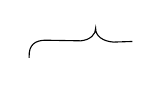
\begin{tikzpicture}[x=.4cm,y=.4cm,baseline=-.2ex]\draw (0,-.34) .. controls (-.03,.10) and (.22,.21) .. (.50,.22)--(1.64,.20) .. controls (1.94,.23) and (2.12,.41) .. (2.11,.60) .. controls (2.10,.35) and (2.35,.18) .. (2.68,.16)--(3.28,.18);\end{tikzpicture}}} that $\underline{G}_m\handwritten{\to}G$ be central\unsure{\handwritten{,}|\handwritten{.}\deleted{,}}\deleted{i.e.}\margin{\deleted{\handwritten{and one \unsure{sees}}}}\inserted{This means\handwritten{
\begin{tikzpicture}[x=.4cm,y=.4cm,baseline=-.2ex]\draw (0,-.40) .. controls (-.08,.05) and (.17,.16) .. (.46,.13)--(2.72,.06) .. controls (2.98,.07) and (3.10,.17) .. (3.11,.42);\end{tikzpicture}}} that the decomp\rlap{i}o\unsure{\rlap{o}s|\rlap{e}s}\rlap{t}ition of an $M$ into \deleted{homogeneous}\inserted{even and odd\handwritten{\unsure{s}}\handwritten{
\begin{tikzpicture}[x=.4cm,y=.4cm,baseline=-.2ex]\draw (0,-.20)--(2.20,-.26) .. controls (2.42,-.26) and (2.58,-.12) .. (2.57,.04);\end{tikzpicture}}} components be invariant under $G$ i.e. take place in $C$,\rlap{e}resp. that the same hold for the decomposition into \inserted{\handwritten{integer}\handwritten{\begin{tikzpicture}[x=.4cm,y=.4cm,baseline=-.2ex]\draw (0,-.30) .. controls (.15,.08) and (.35,.14) .. (.53,.14)--(1.92,.12) .. controls (2.12,.13) and (2.23,.25) .. (2.20,.42);\end{tikzpicture}}} degrees. Note that this last condition is expressed directly in terms of $C$ (equipped with its $\otimes$ structure and the \deleted{forgetful} graded functor\deleted{\unsure{f|s|x}} $C\handwritten{\to}\mathrm{Grdf}(k)$), \deleted{and one \deleted{hopes}\inserted{\handwritten{sees}} that this condition is sufficient (perhaps necessary and sufficient)\inserted{\handwritten{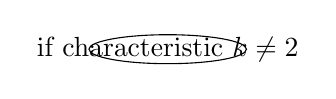
\begin{tikzpicture}[x=.4cm,y=.4cm,baseline=-.2ex]\node at (0,0) {if characteristic $k\ne2$};\draw (0,0) ellipse (2.5 and .46);\end{tikzpicture}}} for one to be in the favourable case\inserted{\handwritten{where}\handwritten{\begin{tikzpicture}[x=.4cm,y=.4cm,baseline=-.2ex]\draw (0,.15) .. controls (.35,.21) and (.56,.13) .. (.64,-.18) .. controls (.70,-.36) and (.91,-.40) .. (1.14,-.40);\end{tikzpicture}}} $C\handwritten{\to}\mathrm{Rep}_k(G)$ \unsure{\rlap{\handwritten{is}}be|be|is} an equivalence.}
\margin{\handwritten{\begin{tikzpicture}[x=.4cm,y=.4cm,baseline=-.2ex]\draw (.18,.42) .. controls (-.05,.46) and (-.08,.25) .. (.01,.02) .. controls (.13,-.30) and (.44,-.34) .. (.68,-.27);\end{tikzpicture}}}


% source lines 19--27
\handwritten{1\unsure{\rlap{-}0|0})} This result will then apply, in particular, to the category of \inserted{s\rlap{m}emi-simple\handwritten{\begin{tikzpicture}[x=.4cm,y=.4cm,baseline=-.2ex]\draw (0,-.40) .. controls (-.05,.06) and (.16,.17) .. (.45,.18)--(2.63,.15) .. controls (2.88,.16) and (3.03,.29) .. (3.02,.49);\end{tikzpicture}}} motives (for the \deleted{functors} natural gradings on the functors $H^\bullet$ which one manages to define there \deleted{are} come from a grading of the category of motives, - which is only a translation of the fact that the \inserted{cohomological\handwritten{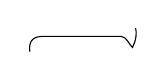
\begin{tikzpicture}[x=.4cm,y=.4cm,baseline=-.2ex]\draw (0,-.34) .. controls (-.05,.05) and (.16,.14) .. (.42,.14)--(2.90,.14) .. controls (3.08,.13) and (3.15,-.12) .. (3.26,-.21) .. controls (3.38,.03) and (3.40,.25) .. (3.36,.40);\end{tikzpicture}}} Kunneth correspondences on a smooth projective algebraic variety are algebraic). One \rlap{e}breathes ! But one will note that the functors $H^\bullet$ in question are not fibre functors properly speaking, but twisted fibre functors.(One will not be able to help calling them fibre functors all the same!) When one works with motives not necess\rlap{i}arily
